\section{Some Linear Time Series Models}
This chapter introduces various probability models for time series. Some tools for describing the properties of 
such models are specified and the important notion of stationarity is formally defined.


% ----------3.1----------
\subsection{Stochastic Processes and Their Properties}
\begin{definition*}[]
A \underline{stochastic process} is a collection of random variables that are ordered in time and defined at a 
set of time points, which may be continuous or discrete. We denote it as $X(t)$ if time is continous, and $X_t$ 
if time is discrete.
\end{definition*}

\begin{definition*}[]
The \underline{mean function} $\mu(t)$ is defined for all $t$ by 
\[ \mu(t) = \mathbb{E}\left[ X(t) \right]. \]
The \underline{variance function} $\sigma^2(t)$ is defined for all $t$ by 
\[ \sigma^2(t) = \mathrm{Var}(X(t)) = \mathbb{E}\left[ (X(t) - \mu(t))^2 \right]. \]
The \underline{autocovariance function (acv.f.)} $\gamma(t_1, t_2)$ is simply the covariance of $X(t_1)$ and $X(t_2)$, namely 
\[ \gamma(t_1, t_2) = \mathbb{E}\left[ (X(t_1) - \mu(t_1))(X(t_2) - \mu(t_2)) \right]. \]
\end{definition*}

Higher moments of a stochastic process may be defined in a similar way, but are rarely used in practice.



% ----------3.1----------
\subsection{Stationary Processes}
An important class of stochastic processes are those that are stationary.

\begin{definition*}[]
A time series is \underline{strictly stationary} if the joint distribution of $X(t_1), \dots, X(t_k)$ is the same as the joint distribution of $X(t_1 + \tau), \dots, X(t_k + \tau)$ for any $t_1, \dots, t_k, \tau$.
\end{definition*}

The definition above for $k = 1$ implies that the distribution of $X(t)$ is the same for all $t$, hence 
\[ \mu(X(t)) = \mu, \sigma^2(X(t)) = \sigma^2 \]
do not depend on the time $t$.

Furthermore, for $k = 2$, the joint distribution of $X(t_1)$ and $X(t_2)$ depends on only the time difference $t_2 - t_1 = \tau$, which is called the \underline{lag}. Thus the acv.f. $\gamma(t_1, t_2)$ only depends on the lag $\tau$ and can be written as $\gamma(\tau)$, where
\begin{align*}
	\gamma(\tau) 
	&= \mathbb{E}\left[ (X(t) - \mu)(X(t+\tau) - \mu) \right] \\
	&= \mathrm{Cov}(X(t), X(t+\tau))
\end{align*}
is the autocovariance function at lag $\tau$.

\begin{definition*}[]
The \underline{autocorrelation function (ac.f.)} is defined by 
\[ \rho(\tau) = \gamma(\tau) / \gamma(0). \]
\end{definition*}
This quantity measures the correlation between $X(t)$ and $X(t+\tau)$.

It may seem surprising to suggest that there are processes for which the distribution of $X(t)$ is the same for 
all $t$. However, from the theory of stochastic processes, there are many processes $\{ X(t) \}$ for which have 
an equilibrium distribution as $t \to \infty$. Of course, the conditional distribution of $X(t_2)$ given $X(t_1)$ 
can be very different, but this does not conflict with the series being stationary.

In practice, it is often useful to define stationarity in a less restricted way:
\begin{definition*}[]
A stochastic process is called \underline{second-order stationary} or \underline{weakly stationary} if its mean 
is constant and its acv.f. only depends on the lag, so that 
\[ \mathbb{E}\left[ X(t) \right] = \mu \text{ and } \mathrm{Cov}(X(t), X(t + \tau)) = \gamma(\tau). \]
\end{definition*}
No requirements are placed on moments higher than the second order. By letting $\tau = 0$, the form of a 
stationary acv.f. implies that the variance, as well as the mean, is constant. The definition also implies that 
both the variance and the mean must be finite.

By stationary, we will mean `weakly stationary' from now on.



% ----------3.3----------
\subsection{Properties of the Autocorrelation Function}
We'll introduce a few general properties of the ac.f. in this subsection.

Suppose a stationary process $X(t)$ has mean $\mu$, variance $\sigma^2$, acv.f. $\gamma(t)$ and ac.f. $\rho(t)$. 
Then 
\[ \rho(t) = \gamma(t) / \gamma(0) = \gamma(t) / \sigma^2. \]
Note that $\rho(0) = 1$.

\begin{proposition*}[Properties of the ac.f.]
For the autocorrelation function $\rho(\tau)$, 
\begin{enumerate}
	\item The ac.f. is an even function of lag, so that $\rho(\tau) = \rho(-\tau)$;
	\item $|\rho(t)| \leq 1$;
	\item The ac.f. does not uniquely identify the underlying model.
\end{enumerate}
\end{proposition*}

\begin{proof}
(i) 
\begin{align*}
	\gamma(\tau) 
	&= \mathrm{Cov}(X(t), X(t + \tau)) \\
	&= \mathrm{Cov}(X(t - \tau), X(t)) \quad \text{(By stationarity)} \\
	&= \gamma(-\tau).
\end{align*}

(ii) First of all, 
\[ \mathrm{Var}(\lambda_1 X(t) + \lambda_2 X(t + \tau)) \geq 0 \]
for any constants $\lambda_1, \lambda_2$, since the variance is always nonnegative. We can expand the above:
\begin{align*}
	\mathrm{Var}(\lambda_1 X(t) + \lambda_2 X(t + \tau))
	&= \lambda_1^2 \mathrm{Var}(X(t)) + \lambda_2^2 \mathrm{Var}(X(t + \tau)) 
	+ 2 \lambda_1 \lambda_2 \mathrm{Cov}(X(t), X(t + \tau)) \\
	&= (\lambda_1^2 + \lambda_2^2)\sigma^2 + 2 \lambda_1 \lambda_2 \gamma(\tau).
\end{align*}
When $\lambda_1 = \lambda_2 = 1$, $\gamma(\tau) \geq -\sigma^2$ so that $\rho(\tau) \geq -1$.

When $\lambda_1 = 1, \lambda_2 = -1$, $\sigma^2 \geq \gamma(\tau)$, so that $\rho(t) \leq +1$.

(iii) An example is given in Jenkins and Watts (1968, p.170). The proof is complete.

\end{proof}

For the ac.f. to guarantee uniqueness of the underlying model, we would also need the invertibility condition, 
which will be introduced in Section 3.6.



% ----------3.4----------
\subsection{Purely Random Process}
\begin{definition*}[]
A discrete-time process is called a \underline{purely random process} or \underline{white noise} if it consists 
of a sequence of random 
variables, $\{ Z_t \}$, which are mutually independent and identically distributed.
\end{definition*}
We normally further assume that the random variables are normally distributed with mean zero and variance 
$\sigma_Z^2$.

From definition, the process has constant mean and variance. Moreover, the independence assumption gives 
\[ \gamma(k) = \mathrm{Cov}(Z_t, Z_{t+k}) = \begin{cases}
	\sigma_Z^2 &\text{ if } k = 0, \\
	0 &\text{ if } k = \pm 1, \pm 2, \dots
\end{cases} \]
Therefore the ac.f. is given by 
\[ \rho(k) = \begin{cases}
	1 &\text{ if } k = 0, \\
	0 &\text{ if } k = \pm 1, \pm 2, \dots
\end{cases} \]

\begin{figure}[h]
	\centering
	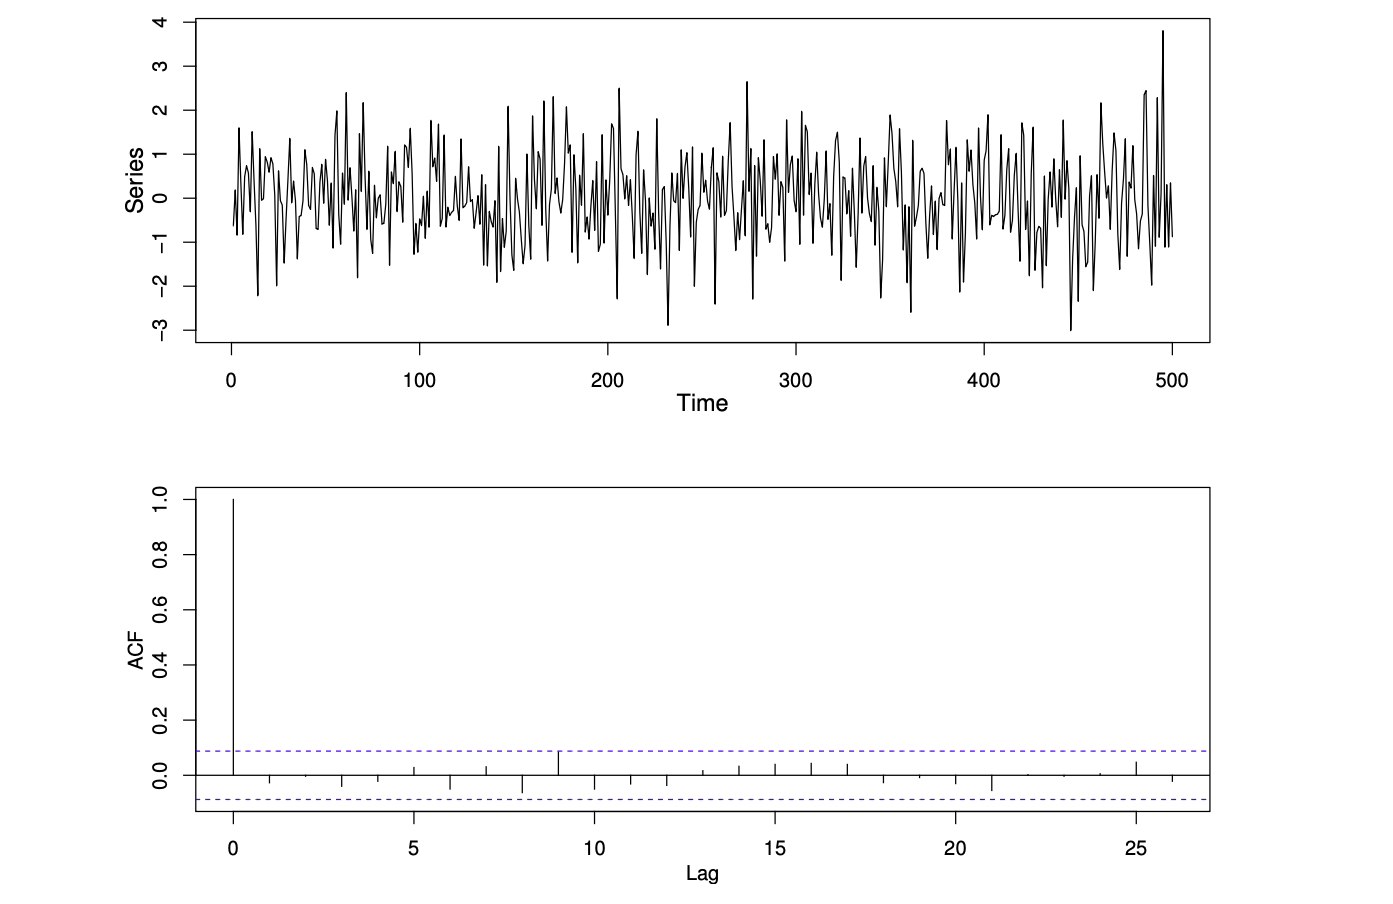
\includegraphics[width=\textwidth]{Chapter 3/fig3-1}
	\caption{A purely random process iwith $\sigma_Z^2 = 1$ (top) and its correlogram (bottom).}
	\label{fig:3.1}
\end{figure}

As the mean and acv.f. do note depend on time, the process is weakly stationary. In fact, the independence 
assumption implies that it is strictly stationary.

Purely random processes are useful in many situations, particularly as building blocks for more complicated 
processes such as moving average processes (Section 3.6). In practice, if all sample ac.f.'s of a series are 
close to zero, then the series is considered as a realization of a purely random process. \cref{fig:3.1} shows 
an example where $Z_t \sim N(0, 1)$, $1 \leq t \leq 500$, and its correlogram, which can be reproduced via the 
following piece of code:
\begin{minted}{R}
> z<-rnorm(500, 0, 1)
> par(mfrow=c(2,1), mar=c(3,4,3,4))
> plot(z, type="l", xlab="Time", ylab="Series")
> acf(z, xlab="Lag",ylab="ACF", main="")
\end{minted}

Some authors prefer to make the weaker assumption that the $Z_t$'s are mutually uncorrelated rather than 
independent. This is fine for linear, normal processes, but not ok for nonlinear models. 



% ----------3.5----------
\subsection{Random Walks}
\begin{definition*}[]
Suppose $\{ Z_t \}$ is a discrete-time, purely random process with mean $\mu$ and variance $\sigma_Z^2$. A 
process $\{ X_t \}$ is said to be a \underline{random walk} if 
\[ X_t = X_{t-1} + Z_t = \sum_{i = 1}^{t} Z_i, \text{ and } X_0 = 0. \]
\end{definition*}

We can easily see that by independence of $Z_t$, 
\[ \mathbb{E}\left[ X_t \right] = t \mu \text{ and } \mathrm{Var}(X_t) = t \sigma_Z^2. \]

As the mean and variance changes with $t$, this process is not stationary. However, by taking the first 
differences, we get 
\[ \nabla X_t = X_t - X_{t-1} = Z_t,  \]
which is stationary. \cref{fig:3.2} below shows a random walk series and its correlogram. 

\begin{figure}[h]
	\centering
	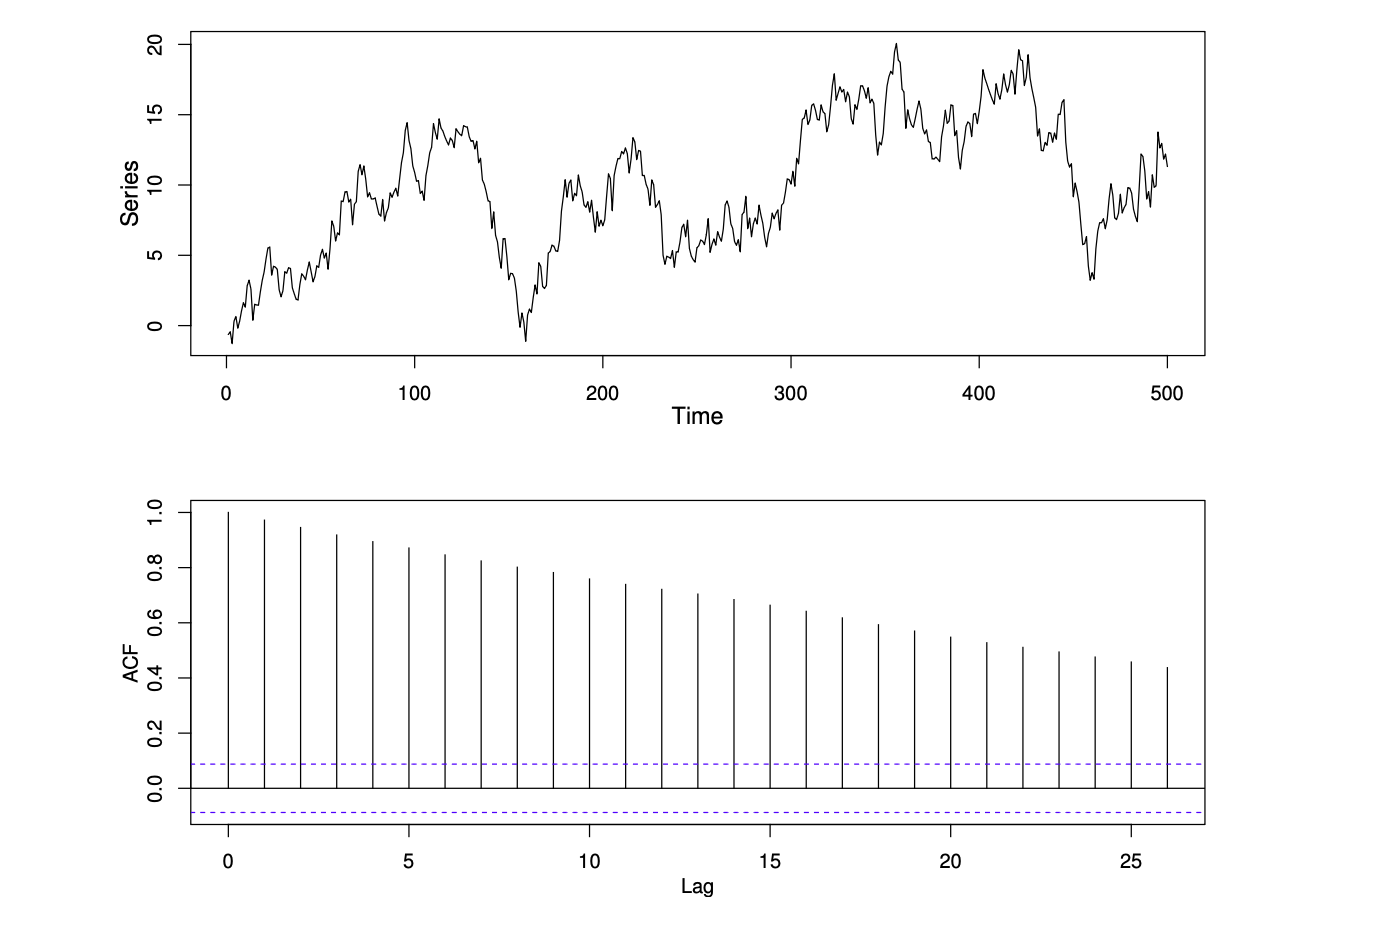
\includegraphics[width=\textwidth]{Chapter 3/fig3-2.png}
	\caption{Simulated random walk (top) and its correlogram (bottom). The random walk series is generated from 
	the white noise series in \cref{fig:3.1}.}
	\label{fig:3.2}
\end{figure}

We can generate the random walk series via the cumulative sum of white noise series using the code below:
\begin{minted}{R}
> n<-500
> z<-rnorm(n, 0, 1)
> x.rw<-cumsum(z)
> par(mfrow=c(2,1), mar=c(4,4,4,4))
> plot(x.rw, type="l", xlab="Time", ylab="Series")
> acf(x.rw, xlab="Lag", ylab="ACF", main="")
\end{minted}
The best-known examples of time series which behave like random walks are share prices.



% ----------3.6----------
\subsection{Moving Average Processes}
\begin{definition*}[]
Suppose $\{ Z_t \}$ is a discrete-time, purely random process with mean zero and variance $\sigma_Z^2$. A 
process $\{ X_t \}$ is said to be a \underline{moving average process of order $q$}, denoted a $\mathrm{MA}(q)$ 
process, if 
\[ X_t = \beta_0Z_t + \beta_1Z_{t-1} + \cdots + \beta_qZ_{t-q}, \]
where $\{ \beta_i \}$ are constants. The $Z$s are usually scaled so that $\beta_0 = 1$.
\end{definition*}


\subsubsection{Stationarity and autocorrelation of an MA process}
We can immediately get that 
\[ \mathbb{E}\left[ X_t \right] = 0, \ \mathrm{Var}(X_t) = \sigma_Z^2 \sum_{i = 0}^{q}\beta_i^2, \]
since the $Z$'s are independent. We also have 
\begin{align*}
	\gamma(k) 
	&= \mathrm{Cov}(X_t, X_{t+k}) \\
	&= \mathrm{Cov}(\beta_0Z_t + \cdots + \beta_q Z_{t-q}, \beta_0Z_{t+k} + \cdots + \beta_qZ_{t+k-q}) \\
	&= \begin{cases}
		0 &\text{ if } k > q, \\
		\sigma_Z^2 \sum_{i = 0}^{q - k} \beta_i \beta_{i+k} &\text{ if } k = 0, 1, \dots, q \\
		\gamma(-k) &\text{if} k < 0
	\end{cases}
\end{align*}
since 
\[ \mathrm{Cov}(Z_s, Z_t) = \begin{cases}
	\sigma_Z^2 &\text{ if } s = t, \\
	0 &\text{ if } s \neq t.
\end{cases} \]
We can see from above that the process is weakly stationary for all values of $\{ \beta_i \}$. Furthermore, if 
the $Z$s are normally distributed, then so are the $X$s, and we have a strictly stationary normal process.

The ac.f. of the $\mathrm{MA}(q)$ process is 
\[ \rho(k) = \begin{cases}
	1 &\text{ if } k = 0, \\
	\frac{\sum_{i = 0}^{q-k}\beta_i \beta_{i+k}}{\sum_{i = 0}^{q}\beta_i^2} &\text{ if } k = 1, \dots, q, \\
	0 &\text{ if } k > q, \\
	\rho(-k) &\text{ if } k < 0.
\end{cases} \]
Note that the ac.f. `cuts off' at lag $q$, which is special of the MA process. In particular, the 
$\mathrm{MA}(1)$ process with $\beta_0 = 1$ has an ac.f. given by 
\[ \rho(k) = \begin{cases}
	1 &\text{ if } k = 0 \\
	\beta_1 / (1 + \beta_1^2) &\text{ if } k = \pm 1 \\
	0 &\text{otherwise.}
\end{cases} \]

Using the definition of the $\mathrm{MA}(q)$ process, we can construct a MA series. For example, \cref{fig:3.3} 
shows the series and their correlograms of these two MA processes:
\[ X_t = Z_t - 0.8Z_{t-1}, Z_t = Z_t + 0.7Z_{t-1} - 0.2Z_{t-2}. \]

\begin{figure}[ht]
	\centering
	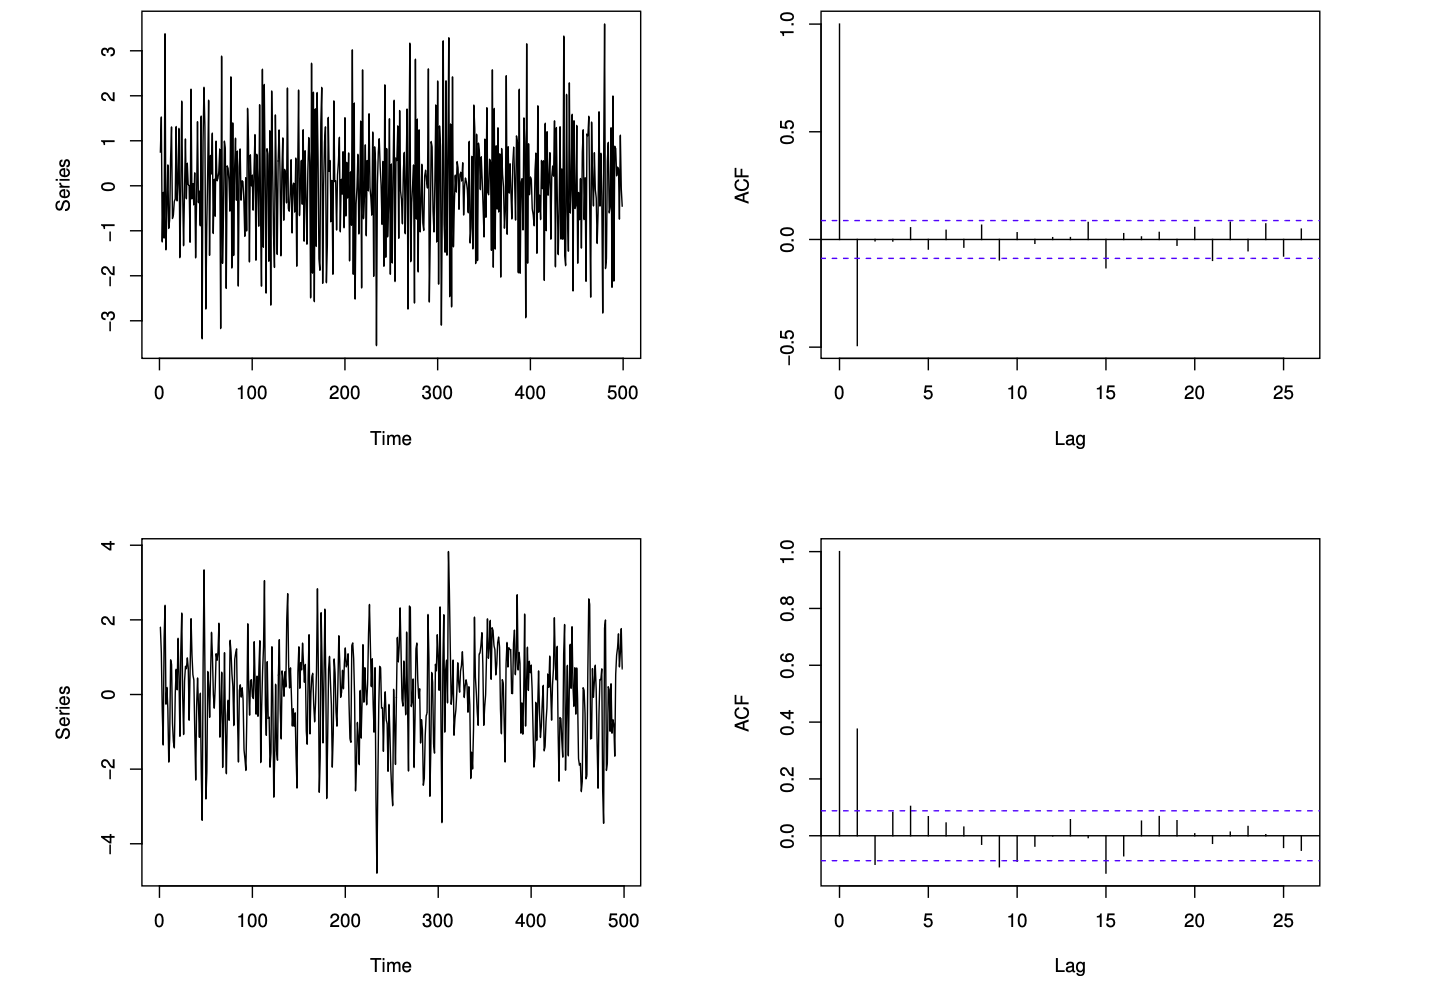
\includegraphics[width=\textwidth]{Chapter 3/fig3-3.png}
	\caption{Simulated MA(1) (top left) and MA(2) (bottom left) processes and their corresponding correlograms 
	(top right and bottom right).}
	\label{fig:3.3}
\end{figure}

We can reproduce \cref{fig:3.3} via the following piece of code:
\begin{minted}{R}
> n<-500
> z<-rnorm(n)
> x.ma1<-z[2:n]-0.8*z[1:(n-1)]
> x.ma2<-z[3:n]+0.7*z[2:(n-1)]-0.2*z[1:(n-2)]

> par(mfrow=c(2,2), mar=c(4,4,4,4))
> plot(x.ma1, type="l", xlab="Time", ylab="Series")
> acf(x.ma1, xlab="Lag", ylab="ACF", main="")
> plot(x.ma2, type="l", xlab="Time", ylab="Series")
> acf(x.ma2, xlab="Lag", ylab="ACF", main="")
\end{minted}

Note that the $r_k$'s are significant only for $k = 0,1$ and $k = 0,1,2$ respectively.


\subsubsection{Invertibility of an MA process}
No restrictions on the $\{ \beta_i \}$ are required for a (finite-order) MA process to be stationary, but it is 
generally advisable to impose restrictions on $\{ \beta_i \}$ so that the process satisfies a condition called 
invertibility. This condition can be explained in the following way. Considering the following MA processes:
\begin{align*}
	\mathrm{A}: \quad & X_t = Z_t + \theta Z_{t-1}. \\
	\mathrm{B}: \quad & X_t = Z_t + \frac{1}{\theta} Z_{t-1}. \\
\end{align*}
Using the formula of the ac.f. for a MA(1) process, we can get that the two different processes have exactly the 
same ac.f. Therefore we cannot identify a MA process uniquely from a given ac.f. Now, if we `invert' models A 
and B by expressing $Z_t$ in terms of $X_t, X_{t-1}, \dots$ via successive substitution, we get that 
\begin{align*}
	\mathrm{A}: \quad & Z_t = X_t - \theta X_{t-1} + \theta^2 X_{t-2} - \cdots \\
	\mathrm{B}: \quad & Z_t = X_t - \frac{1}{\theta} X_{t-1} + \frac{1}{\theta^2} X_{t-2} - \cdots \\
\end{align*}
Of $|\theta| < 1$, the series of coefficients of $X_{t-j}$ for model A converges whereas that of B does not. 
Thus model B cannot be `inverted' this way.

\begin{definition*}[]
A process $\{ X(t) \}$ is said to be \underline{invertible} if the random disturbance at time $t$, sometimes 
called the \textit{innovation}, can be expressed as a convergent sum of present and past values of $X_t$ in the 
form 
\[ Z_t = \sum_{j = 0}^{\infty} \pi_j X_{t-j}, \ \sum_{j}^{} |\pi_j| < \infty. \]
\end{definition*}
Therefore this means a first order MA process can be rewritten in the form of an autoregressive process, 
possible of infinite order, whose coefficients form a convergent sum.

\begin{definition*}[]
The \underline{backshift operator}, denoted $B$, is defined by 
\[ B^j X_t = X_{t-j} \text{ for } j = 0, 1, \dots \]
\end{definition*}

Then the MA process can be rewritten as 
\begin{align*}
	X_t 
	&= (\beta_0 + \beta_1 B + \cdots + \beta_q B^q) Z_t \\
	&= \theta(B) Z_t
\end{align*}
where $\theta(q)$ is a polynomial of order $q$ in $B$.

\begin{theorem*}[Invertibility criterion for MA process]
A $\mathrm{MA}(q)$ process is invertible if the roots of the equation 
\[ \theta(B) = \beta_0 + \beta_1 B + \cdots + \beta_q B^q = 0 \]
all lie outside the unit circle, where we regard $B$ as a complex variable.
\end{theorem*}

\begin{proof}
First of all, from the MA equation we can directly get that 
\[ Z_t = \frac{1}{\theta(B)}X_t. \]
Suppose that $\theta(B)$ can be decomposed into the following form:
\[ \theta(B) = (1 + \theta_1 B) \cdots (1 + \theta_q B), \]
where $\theta_1, \dots, \theta_q$ could possibly take complex variables. Then the operator $1 / \theta(B)$ can 
be written as 
\[ \frac{1}{\theta(B)} = \prod_{j = 1}^{q} \frac{1}{1 + \theta_j B} 
= \prod_{j = 1}^{q} \left( 1 + \sum_{i = 1}^{\infty} (-\theta_j)^i B^i \right). \]
When all the roots, $-1/\theta_1, \dots, -1/\theta_q$, are outside the unit circle, the product on the right 
hand side above is convergent, hence we can indeed write $Z_t = 1 / \theta(B) X_t$, and therefore $\{ X_t \}$ 
is invertible.
\end{proof}

MA processes have been used in many areas, particularly econometrics. For example, economic indicators are 
affected by a variety of `random' events such as strikes, government decisions, shortages of key materials, and 
so on. Such events will not only have an immediate effect but may also affect economic indicators to a lesser 
extent in several subsequent periods, and so it is at least plausible that an MA process may be appropriate.

An arbitrary constant, say $\mu$, can be added to the MA equation to give a process of mean $\mu$. However, 
this does not affect the ac.f. (Exercise 3.5) hence has been omitted.



% ----------3.7----------
\subsection{Autoregressive Processes}
Autoregressive processes are slightly different from moving average processes, but they are closely related 
to each other.

\begin{definition*}[]
Suppose $\{ Z_t \}$ is a discrete-time, purely random process with mean zero and variance $\sigma_Z^2$. A 
process $\{ X_t \}$ is said to be a \underline{autoregressive process of order $p$}, denoted a $\mathrm{AR}(P)$ 
process, if 
\[ X_t = \alpha_1 X_{t-1} + \cdots + \alpha_p X_{t-p} + Z_t. \]
\end{definition*}


\subsubsection{First-order process}
We begin by examining the case where $p = 1$, i.e.
\[ X_t = \alpha X_{t-1} + Z_t. \]
The AR(1) process is sometimes called the Markov process. By substitution to the equation above, we get 
\begin{align*}
	X_t 
	&= \alpha(\alpha X_{t-2} + Z_{t-1}) + Z_t \\
	&= \alpha^2(\alpha X_{t-3} + Z_{t-2}) + \alpha Z_{t-1} + Z_t \\
	&= \cdots
\end{align*}
Therefore $X_t$ can be expressed as an infinite-order MA process in the form 
\[ X_t = Z_t + \alpha Z_{t-1} + \alpha^2 Z_{t-2} + \cdots \]
provided that $|\alpha| < 1$ so that the sum converges.

This shows that there is a duality between AR and MA processes, which we can in fact see by writing in terms of 
the backshift operator:
\[ (1 - \sigma B)X_t = Z_t, \]
so that 
\begin{align*}
	X_t 
	&= Z_t / (1 - \alpha B) \\
	&= (1 + \alpha B + \alpha^2 B^2 + \cdots) Z_t \\
	&= Z_t + \alpha Z_{t-1} + \alpha^2 Z_{t-2} + \cdots
\end{align*}
When expressed in this form, it is clear that 
\[ \mathbb{E}\left[ X_t \right] = 0, \ 
\mathrm{Var}(X_t) = \sigma_Z^2 (1 + \alpha^2 + \alpha^4 + \cdots) = \frac{\sigma_Z^2}{1 - \alpha^2} \]
provided that $|\alpha| < 1$. The acv.f. is given by 
\begin{align*}
	\gamma(k) 
	&= \mathbb{E}\left[ X_t X_{t+k} \right] \\
	&= \mathbb{E}\left[ (\Sigma \alpha^i Z_{t-i})(\Sigma \alpha^j Z_{t+k-j}) \right] \\
	&= \sigma_Z^2 \sum_{i = 0}^{\infty} \alpha^i \alpha^{k+i} \quad (\text{ for } k \geq 0) \\
	&= \alpha^k \sigma_Z^2 / (1 - \alpha^2) \quad (\text{provided } |\alpha| < 1).
\end{align*}
For $k < 0$, we find $\gamma(k) = \gamma(-k)$. Since $\gamma(k)$ does not depend on $t$, an AR(1) process is 
weakly stationary provided that $|\alpha| < 1$, and the ac.f. is then given by 
\[ \rho(k) = \alpha^k, \ k = 0, 1, 2, \dots \]
To get an even functino defined for all integers $k$, we rewrite the above as 
\[ \rho(k) = \alpha^{|k|}, \ k = 0, \pm 1, \pm 2, \dots \]

Three examples of AR processes are shown in \cref{fig:3.4} for $\alpha = 0.8, -0.8,$ and $0.3$. All three series 
are constructed using the same noise series via the code below:

\begin{figure}[ht]
	\centering
	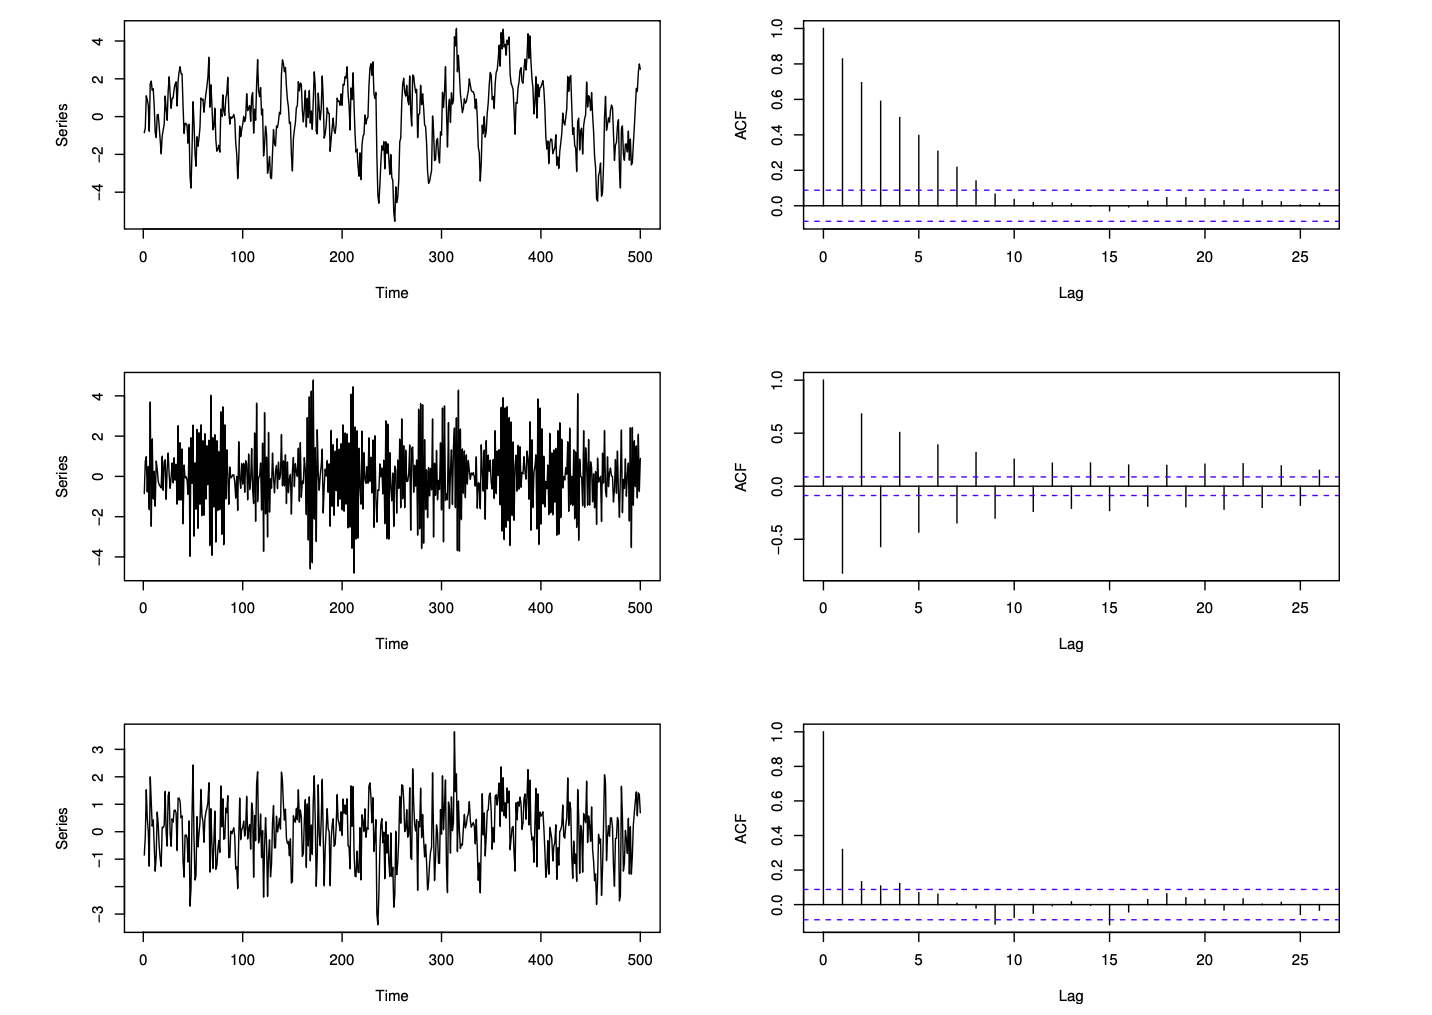
\includegraphics[width=\textwidth]{Chapter 3/fig3-4.png}
	\caption{Three simulated AR(1) processes and their corrolograms. Top: $X_t = 0.8X_{t-1} + Z_t$; Middle: 
	$X_t = -0.8X_{t-1} + Z_t$; Bottom: $X_t = 0.3X_{t-1} + Z_t$, $Z_t \sim N(0, 1)$.}
	\label{fig:3.4}
\end{figure}

\begin{minted}{R}
> n<-500
> z<-rnorm(n, 0, 1)
> x.ar1.1<-x.ar1.2<-x.ar1.3<-rep(0,n)
> x.ar1.1[1]<-x.ar1.2[1]<-x.ar1.3[1]<-z[1]
> for (i in 2:n){
    x.ar1.1[i]<- 0.8*x.ar1.1[i-1]+z[i]
    x.ar1.2[i]<- -0.8*x.ar1.2[i-1]+z[i]
    x.ar1.3[i]<- 0.3*x.ar1.3[i-1]+z[i]
  }
\end{minted}

Note how quick the ac.f. decays when $\alpha = 0.3$, and how it alternates when $\alpha = -0.8$.


\subsubsection{General order process}
Recall the AR equation:
\[ X_t = \alpha_1 X_{t-1} + \cdots + \alpha_p X_{t-p} + Z_t \implies 
(1 - \alpha_1 B - \cdots - \alpha_p B^p) X_t = Z_t. \]
We can rewrite this as 
\[ X_t = Z_t / (1 - \alpha_1 B - \cdots - \alpha_p B^p) = f(B)Z_t, \]
where 
\begin{align*}
	f(B) 
	&= (1 - \alpha_1 B - \cdots - \alpha_p B^p)^{-1} \\
	&= (1 + \beta_1 B + \beta_2 B^2 + \cdots).
\end{align*}
The relationship between the $a$'s and the $\beta$'s may then be found. Since we just rewrote it as an 
$\mathrm{MA}(\infty)$ process, it follows that $\mathbb{E}\left[ X_t \right] = 0$. The variance is finite 
provided that $\sum_{}^{}\beta_i^2$ converges, and is a necessary condition for stationarity. We can rewrite 
the acv.f. by the $\beta$'s:
\[ \gamma(k) = \sigma_Z^2 \sum_{i = 0}^{\infty} \beta_i \beta_{i+k}, \ \beta_0 = 1. \]
A sufficient condition for this to converge, and hence stationarity, is that $\sum_{}^{}|\beta_i|$ converges.

\textit{Yule-Walker equations}
We can in principle find the ac.f. of any $\mathrm{AR}(p)$ process using the above procedure, but the $\beta_i$ 
may be algebraically hard to find. The simpler way is to \textit{assume} the process is stationary, multiply 
through the AR equation by $X_{t-k}$, take expectations and divide by $\sigma_X^2$, assuming that the variance 
of $X_t$ is finite. Then, using the fact that $\rho(k)$ is even, we find:

\begin{definition*}[]
The \underline{Yule-Walker equations} are the following set of linear equations:
\[ \rho(k) = \alpha_1 \rho(k - 1) + \cdots + \alpha_p \rho(k - p) \text{ for all } k = 1, 2, \dots \]
\end{definition*}

It is a set of difference equations and has the general solution 
\[ \rho(k) = A_1 \pi_1^{|k|} + \cdots + A_p \pi_p^{|k|}, \]
where $\{ \pi_i \}$ are the roots of the auxiliary equation 
\[ y^p - \alpha_1 y^{p-1} - \cdots - \alpha_p = 0. \]
The constants $\{ A_i \}$ are chosen to satisfy the initial conditions depending on $\rho(0) = 1$, meaning that 
$\sum_{}^{}A_i = 1$.

\textit{Stationarity conditions}
From the general form of $\rho(k)$, it is clear that $\rho(k)$ tends to zero as $k$ increases provided that 
$|\pi_i| < 1$ for all $i$, and this is a necessary and sufficient condition for the $\mathrm{AR}(p)$ process to 
be stationary. Equivalently, this is equal to the roots of the equation 
\[ \phi(B) = 1 - \alpha_1 B - \cdots - \alpha_p B^p = 0 \]
must lie outside the unit circle.

Of particular interest is the AR(2) process, when $\pi_1, \pi_2$ are the roots of the quadratic equation 
\[ y^2 - \alpha_1 y - \alpha_2 = 0. \]
Here $|\pi_i| < 1$ if 
\[ \left| \frac{\alpha_1 \pm \sqrt{\alpha_1^2 + 4 \alpha_2}}{2} \right| < 1 \]
from which we can show (Exercise 3.6) that the stationarity region is the triangular region satisfying 
\[ \alpha_1 + \alpha_2 < 1, \ \alpha_1 - \alpha_2 > -1, \alpha_2 > -1. \]
The roots are real if $\alpha_1 + 4 \alpha_2 > 0$, in which case the ac.f. decreases exponentially with $k$, but 
the roots are complex if $\alpha_1^2 + 4 \alpha_2 < 0$, in which case the ac.f. turns out to be a damped 
sinusoidal wave.

When the roots are real, $\rho(k) = A_1 \pi_1^{|k|} + A_2 \pi_2^{|k|}$ where the constants $A_1, A_2$ are also 
real and may be found as follows. Since $\rho(0) = 1$, 
\[ A_1 + A_2 = 1 \]
while the first Yule-Walker equation gives 
\begin{align*}
	\rho(1) 
	&= \alpha_1 \rho(0) + \alpha_2 \rho(-1) \\
	&= \alpha_1 + \alpha_2 \rho(1).
\end{align*}
Solving the above gives $\rho(1) = \alpha_1 / (1 - \alpha_2)$, which in turn must equal 
\[ A_1 \pi_1 + A_2 \pi_2 = A_1 \pi_1 + (1 - A_1)\pi_2. \]
Therefore, we finally get 
\[ \begin{cases}
	A_1 &= \frac{\alpha_1 / (1 - \alpha_2) - \pi_2}{\pi_1 - \pi_2} \\
	A_2 &= 1 - A_1
\end{cases} \]
and we can write down the general form of the ac.f. of an AR(2) process with real roots.

For example, consider the AR(2) process defined by $X_t = 1/3X_{t-1} + 2/9X_{t-2} + Z_t$. \cref{fig:3.5} 
below shows a realization of this process and its correlogram. The roots are -3 and 3/2, hence we can use the 
formula above to find its ac.f. (Exercise 3.6).

\begin{figure}[h]
	\centering
	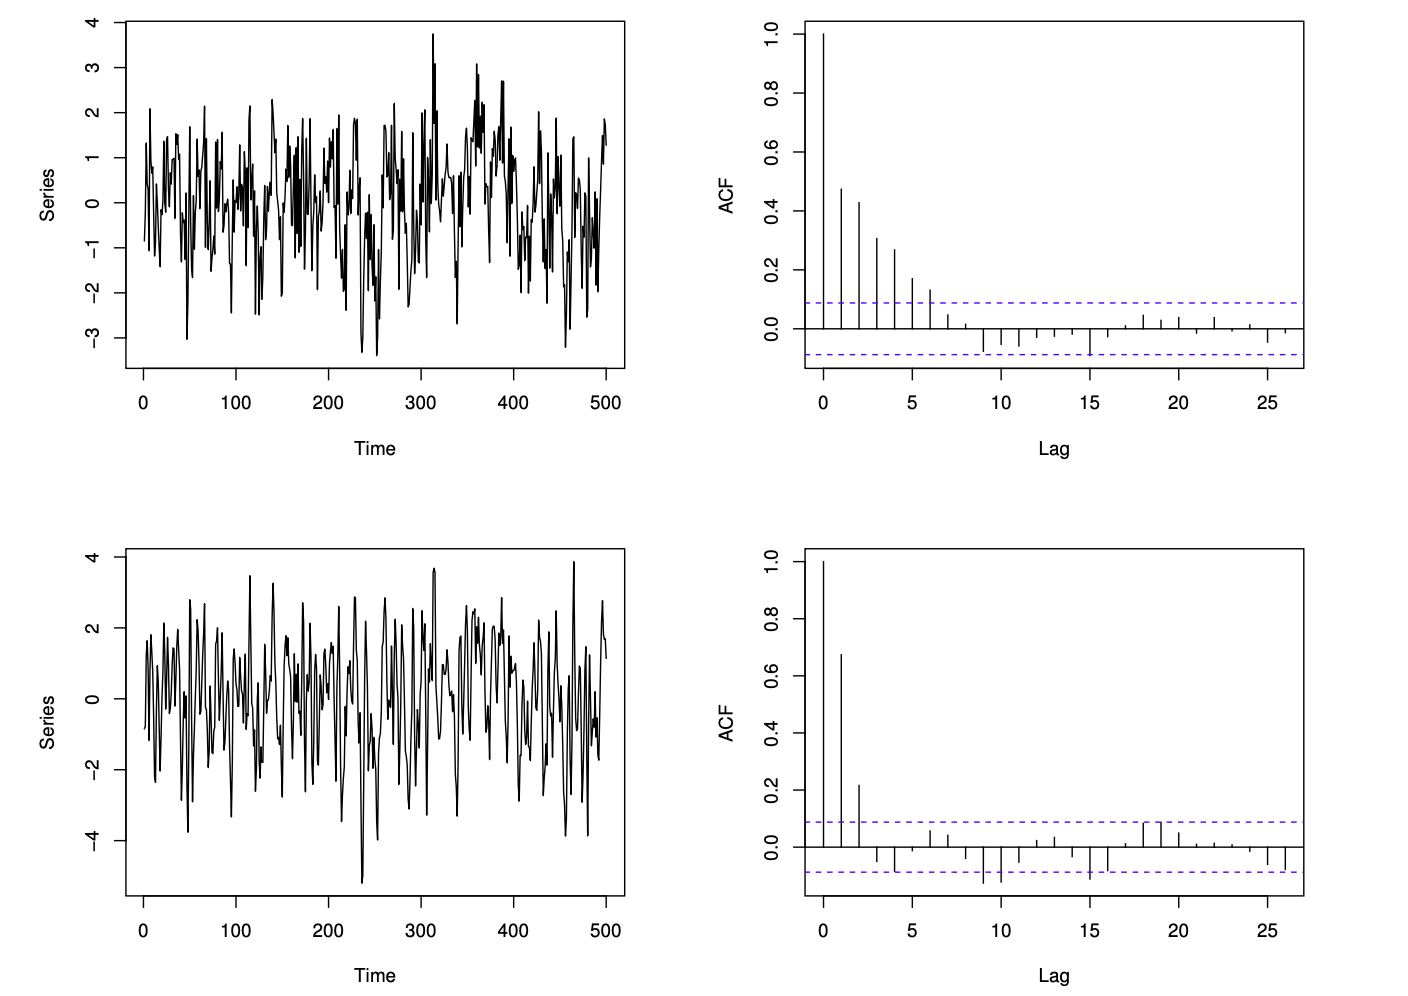
\includegraphics[width=\textwidth]{Chapter 3/fig3-5.png}
	\caption{Two simulated AR(2) processes and their correlograms. Top: $X_t = \frac{1}{3}X_{t-1} + \frac{2}{9} 
	X_{t-2} + Z_t$; Bottom: $X_t = X_{t-1} - \frac{1}{2}X_{t-2} + Z_t$; $Z_t \sim N(0, 1)$.}
	\label{fig:3.5}
\end{figure}

Now let's look at an example for complex roots:
\begin{example}[]
\label{ex:3.1}
Consider the AR(2) process given by 
\[ X_t = X_{t-1} - \frac{1}{2}X_{t-2} + Z_t. \]
Is this process stationary? If so, what is its ac.f.?

Let's look at the roots of the polynomial, in this case, it's
\[ \phi(B) = 1 - B + \frac{1}{2}B^2 = 0. \]
The roots are $1 \pm i$. The modulus of both roots exceed one, hence the process is stationary.

Now, to find the ac.f., we use the first Yule-Walker equation to give 
\begin{align*}
	\rho(1) = \rho(0) - \frac{1}{2}\rho(-1) \\
	&= 1 - \frac{1}{2}\rho(1),
\end{align*}
giving $\rho(1) = 2/3$. 

We can use the Yule-Walker equations to solve for $\rho(2), \rho(3)$ and so on by successive substitution, but 
let's use a smarter approach by solving the set of Yule-Walker equations as a set of difference equations. The 
Yule-Walker equation above has the auxiliary equation 
\[ y^2 - y + \frac{1}{2} = 0 \]
with roots $(1 \pm i)/2$. By Euler's formula, this is 
\[ \frac{1 \pm i}{2} = \frac{\cos{(\pi/4)} \pm i \sin{(\pi/4)}}{\sqrt{2}} = e^{\pm i \pi/4} / \sqrt{2}. \]
Since $\alpha_1^2 + 4 \alpha_2 = 1 - 2 < 0$, and the roots are complex, the ac.f. is a dampled sinusoidal wave. 
Using $\rho(0) = 1$ and $\rho(1) = 2/3$, some messy trigonometry and algebra involving complex numbers gives 
\[ \rho(k) = \left( \frac{1}{\sqrt{2}} \right)^k \left( \cos{\frac{\pi k}{4}} + \frac{1}{3} 
\sin{\frac{\pi k}{4}} \right) \]
for $k = 0, 1, 2, \dots$. Note that the values of the ac.f. are all real even if the roots of the auxiliary 
equation are complex. The bottom two panels of \cref{fig:3.5} show a realization of $X_t$ and its correlogram.
\end{example}

Again, like MA processes, non-zero means may be dealth with by rewriting the AR equation as 
\[ X_t - \mu = \alpha_1 (X_{t-1} - \mu) + \cdots + \alpha_p (X_{t-p} - \mu) + Z_t. \]
This does not affect the ac.f. (Exercise 3.4).



% ----------3.8----------
\subsection{Mixed ARMA Models}
A useful class of models for time series is formed by combining AR and MA processes:
\begin{definition*}[]

A \underline{mixed autoregressive moving average process} containing $p$ AR terms and $q$ MA terms is said to be 
an ARMA process or order $(p, q)$. It is given by 
\[ X_t = \alpha_1 X_{t-1} + \cdots + \alpha_p X_{t-p} + Z_t + \beta_1 Z_{t-1} + \cdots + \beta_q Z_{t-q}, \]
where $\{ Z_t \}$ is a purely random process with mean zero and variance $\sigma_Z^2$.
\end{definition*}

Using the backshift operator, we can rewrite the above as
\[ \phi(B)X_t = \theta(B) Z_t. \]
where $\phi(B), \theta(B)$ are polynomials of order $p,q$ respectively, such that 
\[ \phi(B) = 1 - \alpha_1 B - \cdots - \alpha_p B^p \]
and 
\[ \theta(B) = 1 + \beta_1 B + \cdots + \beta_q B^q. \]


\subsubsection{Stationarity and invertibility conditions}
The conditions to make the process stationary and invertible are those combined for the pure AR and pure MA 
processes. This means the roots for the equation 
\[ \phi(B) = 0, \theta(B) = 0 \]
all lie outside the unit circle. In is straightforward in principle, though algebraically tedious, to calculate 
the ac.f. of an ARMA process. This is not discussed in the text (Exercise 3.11).

The importance of ARMA processes lies in the fact that a stationary time series may often be adequately modelled 
by an ARMA model involving fewer parameters than a pure MA or AR process by itself. This is an early example of
what is often called the Principle of Parsimony. This says that we want to find a model with as few parameters 
as possible, but which gives an adequate representation of the data at hand.


\subsubsection{Yule-Walker equations and autocorrelations}
The ac.f. of an ARMA process can be found using similar procedures as for AR processe. First, multiply through 
the ARMA equation by $X_{t-k}$ and take expectations. Note that, for $k > q$, $Z_t, \dots, Z_{t-q}$ are 
independent of $X_{t-k}$. Hence the expected values of $Z_tX_{t-k}, \dots, Z_{t-q}X_{t-k}$ are all zero. 
If $k \geq p$, we can further divide both sides of the equation by $\gamma(0)$, then we get the Yule-Walker 
equations for the general $\mathrm{ARMA}(p, q)$ process
\[ \rho(k) = \alpha_1 \rho(k-1) + \cdots + \alpha_p \rho(k - p), \ k \geq \max_{}(p, q + 1). \]
Note that the form is the exact same as that of a pure AR process, but the initial conditions are different. 
Here is an example of how to compute the ac.f.:

\begin{example}[]

Consider the $\mathrm{ARMA}(1, 1)$ process
\[ X_t = \alphaX_{t-1} + Z_t + \beta Z_{t-1},  \]
where $|\alpha|, |\beta| < 1$. To derive the ac.f. of the process, the Yule-Walker equations are 
\[ \rho(k) = \alpha \rho(k-1), \ k \geq 2. \]
To obtain the initial conditions, we note that $\gamma(1)$ can be computed as follows:
\begin{align*}
	\gamma(1) 
	&= \mathrm{Cov}(X_t, X_{t-1}) \\
	&= \mathrm{Cov}(\alpha X_{t-1} + Z_t + \beta Z_{t-1}, X_{t-1}) \\
	&= \alpha \gamma(0) + \beta \mathrm{Cov}(Z_{t-1}, X_{t-1}) \\
	&= \alpha \gamma(0) + \beta \mathrm{Cov}(Z_{t-1}, \alpha X_{t-2} + Z_t + \beta Z_{t-2}) \\
	&= \alpha \gamma(0) + \beta \sigma_Z^2.
\end{align*}
The variance of $X_t$, or $\gamma(0)$, can be calculated as follows:
\begin{align*}
	\gamma(0) 
	&= \mathrm{Var}(\alpha X_{t-1} + Z_t + \beta Z_{t-1}) \\
	&= \mathrm{Cov}(\alpha X_{t-1} + Z_t + \beta Z_{t-1}, \alpha X_{t-1} + Z_t + \beta Z_{t-1}) \\
	&= \alpha^2 \gamma(0) + (1 + \beta^2)\sigma_Z^2 + 2 \alpha \beta \mathrm{Cov}(X_{t-1}, Z_{t-1}) \\
	&= \alpha^2 \gamma(0) + (1 + 2 \alpha \beta + \beta^2)\sigma_Z^2.
\end{align*}
Solving for $\gamma(0)$ gives 
\[ \gamma(0) = \frac{1 + 2 \alpha \beta + \beta^2}{1 - \alpha^2} \sigma_Z^2. \]
Thewn plugging this into the equation for $\gamma(1)$ gives 
\[ \gamma(1) = \frac{(1 + \alpha \beta)(\alpha + \beta)}{1 - \alpha^2}\sigma_Z^2. \]
Therefore, 
\[ \rho(1) = \frac{\gamma(1)}{\gamma(0)} = \frac{(1 + \alpha \beta)(\alpha + \beta)}
{1 + 2 \alpha \beta + \beta^2}. \]
USing the Yule-Walker equations, we then have 
\[ \rho(k) = \frac{\gamma(1)}{\gamma(0)} = \frac{(1 + \alpha \beta)(\alpha + \beta)}
{1 + 2 \alpha \beta + \beta^2} \alpha^{k - 1}, \ k \geq 1. \]
\end{example}

\begin{figure}[ht]
	\centering
	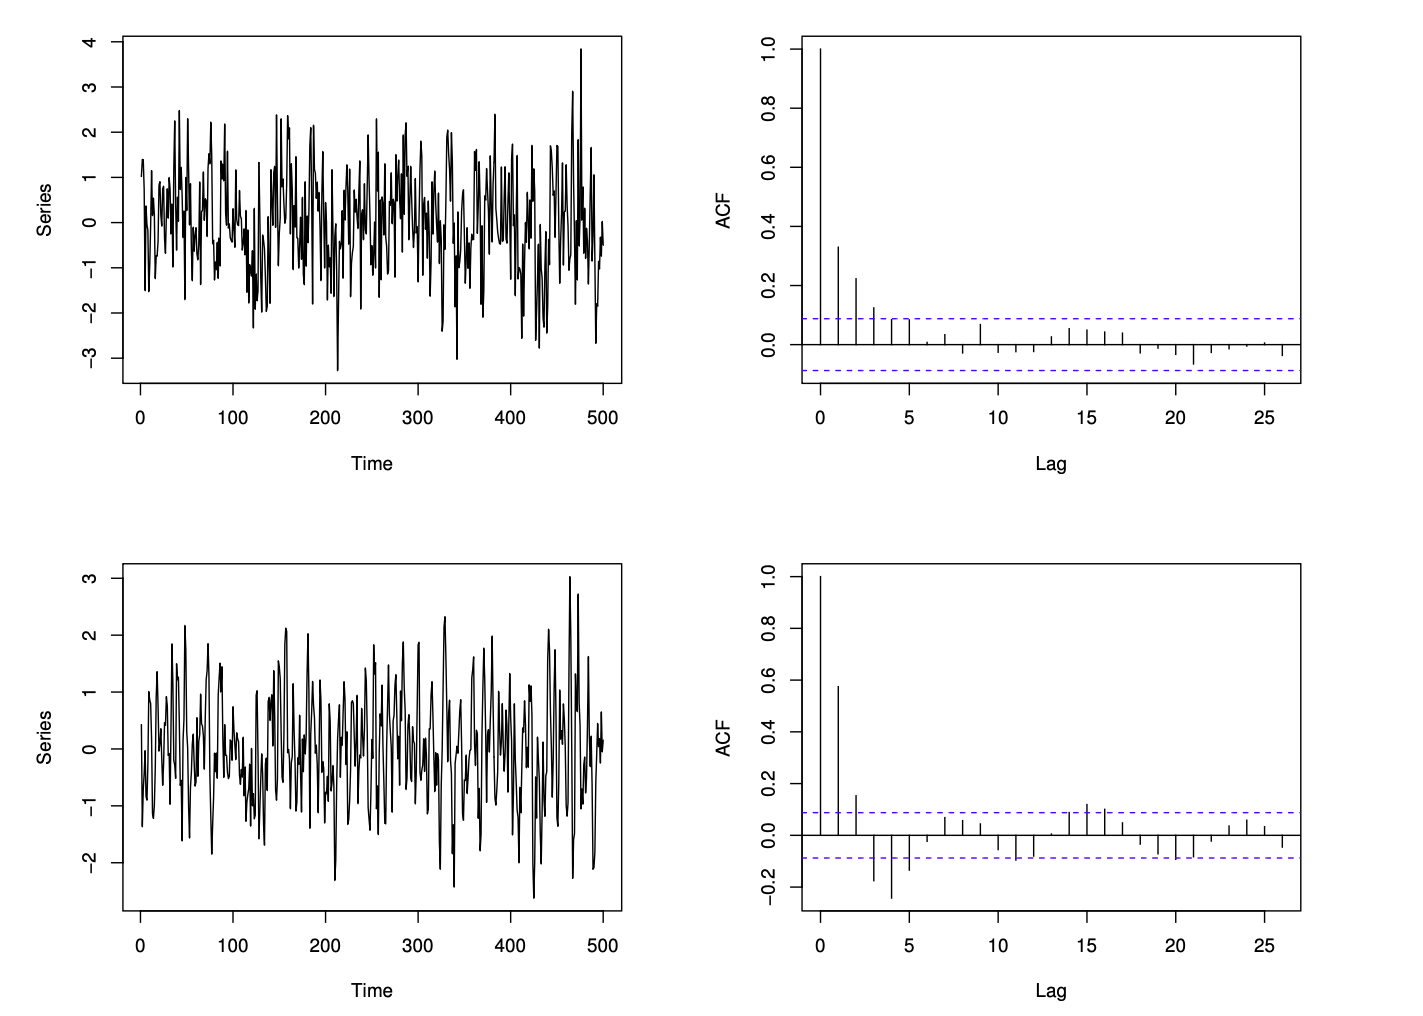
\includegraphics[width=\textwidth]{Chapter 3/fig3-6.png}
	\caption{Two simulated ARMA processes and their correlograms. Top: $X_t = 0.7X_{t-1} + Z_t - 0.4Z_{t-1}$; 
	Bottom: $X_t = 0.9X_{t-1} - 0.5X_{t-2} + Z_t - 0.2Z_{t-1} + 0.25Z_{t-2}$, $Z_t \sim N(0, 0.5)$.}
	\label{fig:3.6}
\end{figure}

In principle, the ac.f. for a general ARMA process can be computed, but are usually more complicated than for 
AR processes. \cref{fig:3.6} above shows two simulated AR processes and their correlograms using the following 
piece of code:
\begin{minted}{R}
> x1<-arima.sim(n=500, list(ar=0.7, ma=-0.4))
> x2<-arima.sim(n=500, list(ar=c(0.9,-0.5), ma=c(-0.2,0.25)), sd=sqrt(0.5))
\end{minted}

Note that, though the correlogram of the ARMA(2, 2) process in \cref{fig:3.6} looks like that from the AR(2) 
process in \cref{fig:3.5}, these processes are completely different!


\subsubsection{AR and MA representations}
We can express ARMA processes as a pure MA process or a pure AR process: 
\[ X_t = \psi(B)Z_t \text{ or } \pi(B) X_t = Z_t, \]
where 
\[ \psi(B) = \sum_{i = 0}^{\infty} \psi_i B^i \text{ and } \pi(B) = 1 - \sum_{i = 1}^{\infty} \pi_i B^i. \]
We can immediately get that
\[ \pi(B) \psi(B) = 1. \]
The weights of $\psi$ or $\pi$ can be obtained directly by division or by equating powers of $B$ in an equation 
such as
\[ \psi(B) \phi(B) = \theta(B). \]

\begin{example}[]
Find the $\psi$ weights and $\pi$ weights for the ARMA(1, 1) process given by 
\[ X_t = 0.5X_{t-1} + Z_t - 0.3Z_{t-1}. \]
Here $\phi(B) = 1 - 0.5B$ and $\theta(B) = 1 - 0.3B$. It follows that the process is stationary and invertible, 
because both equations have roots greter than one. Then 
\begin{align*}
	\psi(B)
	&= \theta(B) / \phi(B) \\
	&= (1 - 0.3B) (1 - 0.5B)^{-1} \\
	&= (1 - 0.3B))(1 + 0.5B + 0.5^2 B^2 + \cdots) \\
	&= 1 + 0.2B + 0.1B^2 + 0.05B^2 + \cdots
\end{align*}
Hence 
\[ \psi_0 = 1, \ \psi_i = 0.2 \times 0.5^{i - 1} \text{ for } i = 1, 2, \dots \]
Similarly, we find 
\[ \pi_0 = 1, \ \pi_i = 0.2 \times 0.3^{i - 1} \text{ for } i = 1, 2, \dots \]
Note that both the $\psi$ and the $\pi$ weights die away quickly, and this also indicates a stationary, 
invertible process.
\end{example}



% ----------3.9----------
\subsection{Integrated ARMA (or ARIMA) Models}
In practice most time series are non-stationary. If the time series is non-stationary in the mean, then we can 
difference the series, as suggested in Section 2.5.3. 

\begin{definition*}[]
Set 
\[ W_t = \nabla^d X_t = (1 - b)^d X_t, \ d = 0, 1, 2, \dots \]
The \underline{autoregressive integrated moving average (ARIMA)} process of order $(p,d,q)$ is of the form
\[ W_t = \alpha_1 W_{t-1} + \cdots + \alpha_pW_{t-p} + Z_t + \beta_1Z_{t-1} + \cdots + \beta_1 Z_{t-q}. \]
\end{definition*}

Of course, we can write the above using backshift operators:
\[ \phi(B) W_t = \theta(B) Z_t \]
or 
\[ \phi(B)(1 - B)^d X_t = \theta(B) Z_t. \]

The model for $X_t$ is clearly non-stationary, as the AR operator has $d$ roots on the unit circle. For example, 
the random walk can be regarded as an ARIMA(0, 1, 0) process, which is non-stationary. Applying the difference 
operator once makes the process stationary.

\cref{fig:3.7} shows a simulated ARIMA(1, 1, 1) and a simmmulated ARIMA(1, 1, 2) process via theh following 
piece of code:
\begin{minted}{R}
> y1<-arima.sim(list(order=c(1,1,1), ar=-0.5, ma=-0.3), n=500)
> y2<-arima.sim(list(order=c(1,1,2), ar=0.3, ma=c(-0.3,0.5)), n=500)
\end{minted}

\begin{figure}[ht]
	\centering
	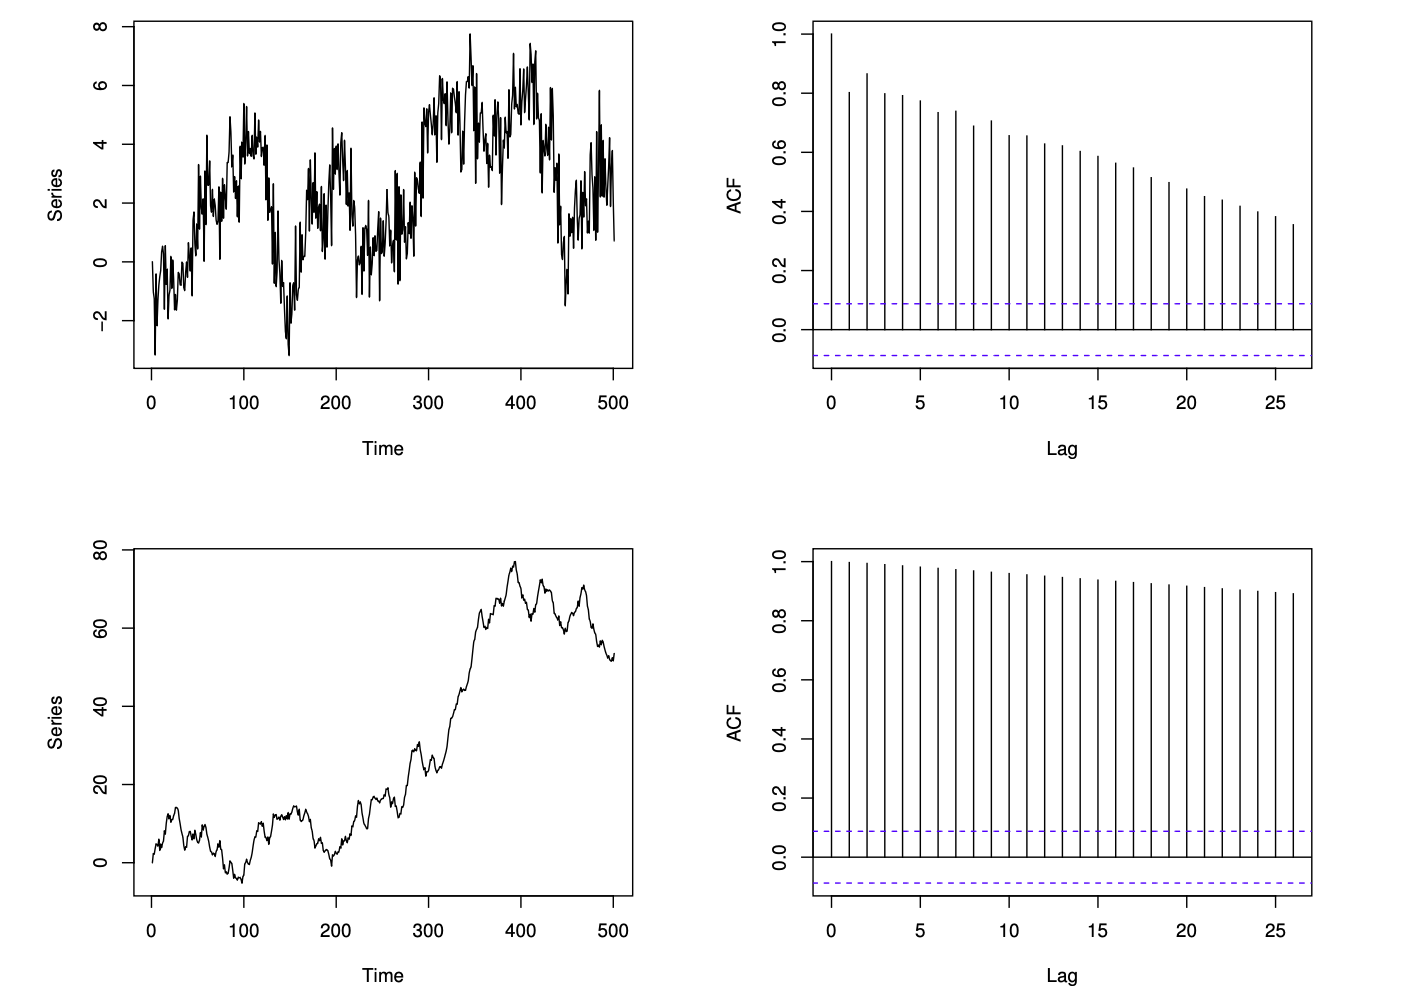
\includegraphics[width=\textwidth]{Chapter 3/fig3-7.png}
	\caption{Two simulated ARIMA processes and their correlograms. Top: $(1 + 0.5B)(1-B)X_t = (1 + 0.3B)Z_t$; 
	Bottom: $(1 - 0.6B)(1 - B)X_t = (1 - 0.3B + 0.5B^2)Z_t$.}
	\label{fig:3.7}
\end{figure}

ARIMA models can be generalized to include seasonal terms, which will be discussed in Section 4.8.



% ----------3.10----------
\subsection{Fractional Differencing and Long-Memory Models}
An interesting variant of ARIMA modeling arises with the use of fractional differencing, leading to a fractional 
integrated ARMA model:
\begin{definition*}[]
A \underline{fractional integrated ARMA (ARFIMA)} process is a process defined by 
\[ \phi(B)(1 - B)^d X_t = \theta(B) Z_t, \]
where $\phi(B)$ and $\theta(B)$ are polynomials of oreder $p, q$ respectively, and $d$ does not need to be an 
integer.
\end{definition*}

When $d$ is not an integer, then the $d$th difference $(1 - B)^d X_t$ becomes a fractional difference, and may 
be represented by its binomial expansion, namely 
\[ (1 - B)^d X_t = \left[ 1 - dB + \frac{d(d - 1)}{2!}B^2 - \frac{d(d-1)(d-2)}{3!}B^3 + \cdots \right] \]
As such, it is an infinite weighted sum of past values.

It can be shown (Brockwell \& Davis, 1991, Section 13.2) that an ARFIMA process is stationary provided that 
$-0.5 < d < 0.5$. For $d > 1/2$, the processes is not stationary in the usual sense, but further integer 
differencing can be used to give a stationary ARFIMA process. For example, first differencing of an 
$\mathrm{ARFIMA}(p, d=1.3, q)$ process gives a stationary $\mathrm{ARFIMA}(p, d=0.3, q)$ process.

A stationary ARFIMA model with $0 < d < 0.5$, is of particular interest as such a process is not only 
stationary, but is also an exmaple of a \textbf{long-memory model}. This means the correlations decay to zero 
very slowly.

\begin{definition*}[]
A stationary process with ac.f. $\rho(k)$ is a \underline{long-memory process} if 
\[ \sum_{k = 0}^{\infty} |\rho(k)| \]
does not converge.
\end{definition*}

In particular, the latter condition applies when the ac.f. is of the form $\rho(k) \sim Ck^{2d - 1}$ as 
$k \to \infty$, where $X$ is a nonzero constant, and $0 < d < 0.5$. It can be shown that a stationary ARFIMA 
model with differencing parameter $d$ in the range $0 < d < 0.5$, as an ac.f. $\rho_k$ whose limiting form has 
the required structure.

As an example, \cref{fig:3.8} shows a simulated $\mathrm{ARFIMA}(1, d=0.4, 2)$ series, 
\[ (1 - 0.3B)(1 - B)^d X_t = (1 - 0.3B + 0.5B^2)Z_t, \ Z_t \sim N(0, 0.2^2), \]
and its correlogram in R. Note that a specific package, fracdiff, needs to be loaded before calling the function 
fracdiff.sim.

\begin{figure}[h]
	\centering
	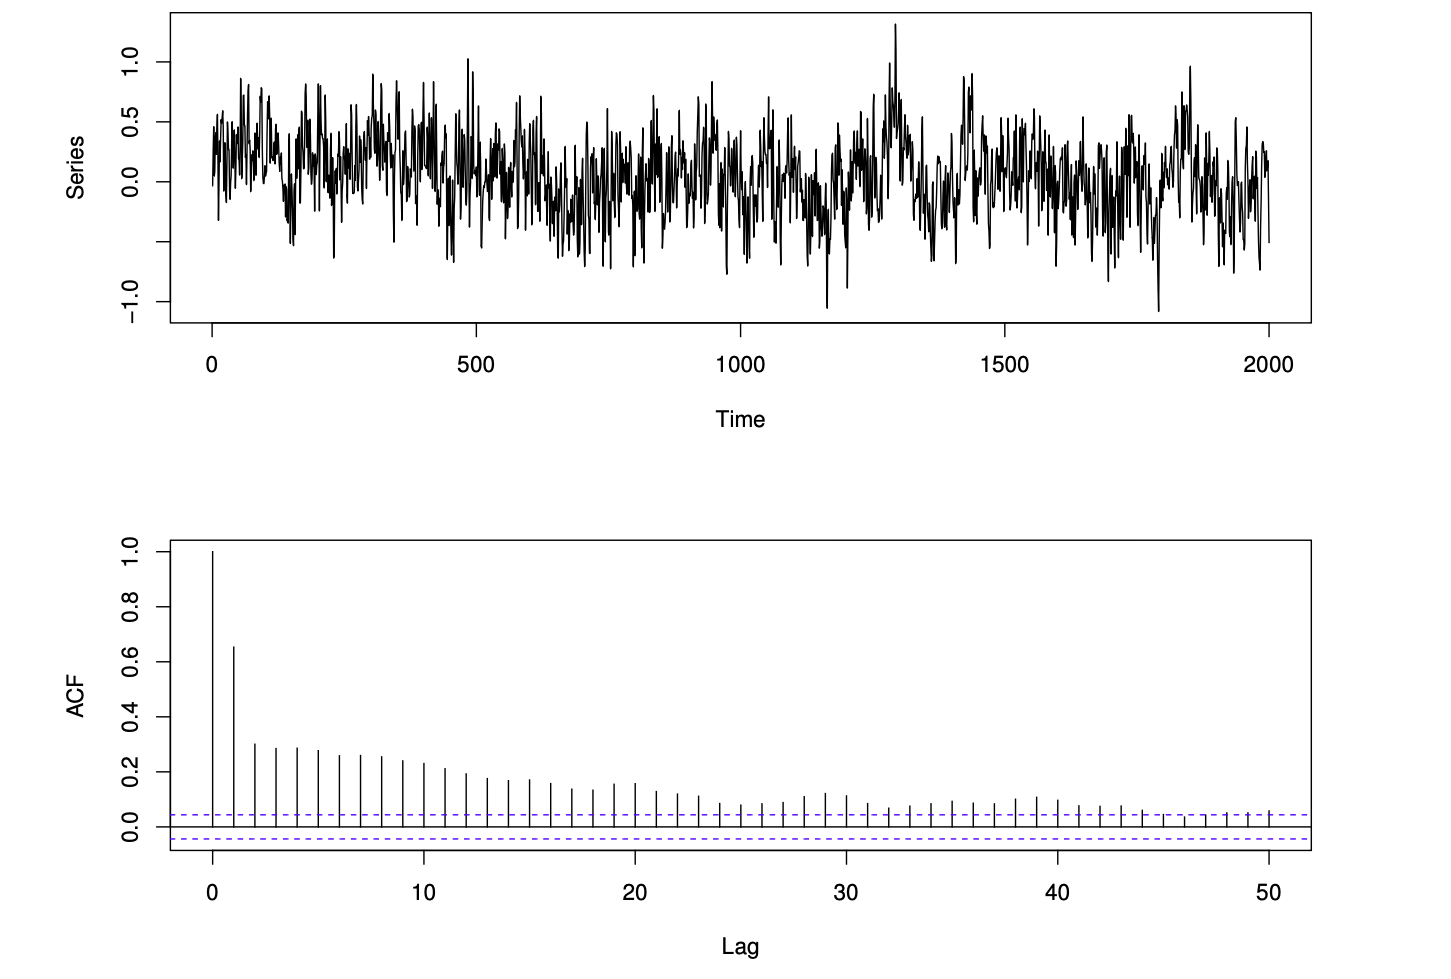
\includegraphics[width=\textwidth]{Chapter 3/fig3-8.png}
	\caption{A simulated $\mathrm{ARFIMA}(1, d=0.4, 2)$ process, $(1 - 0.3B)(1 - B)^d X_t 
	= (1 - 0.3B + 0.5B^2)Z_t$ with $Z_t \sim N(0, 0.04)$, and its correlogram.}
	\label{fig:3.8}
\end{figure}

In contrast, the ac.f. of a stationary ARMA process satisfies the condition that $|\rho(k)| < C \lambda^k$, 
where $C$ is a constant and $0 < \lambda < 1$. Thus there correlations are absolutely summable and such 
processes may be called short-memory models.

Long-memory models have a number of interesting features, especially for forecasting. In time-series analysis, 
the variance of a sample mean can be expressed as 
\[ \frac{\sigma_Z^2}{N} [1 + 2 \sum_{k = 1}^{N - 1} \left( 1 - \frac{k}{n} \right) \rho(k)]; \]
see Section 4.1.2. When the correlationas are positive, as they usually are, the latter expression can be much 
larger then $\sigma^2 / N$, especially for long-memory processes where the correlations die out slowly. In 
contrast to this result, it is intuitively clear that the larger and longer lasting the autocorrelations, the 
better will be the forecasts of the model. It can be shown both theoretically and practically (Bera, 1994, 
Section 8.7), but is not shown in this book.

\textit{A long-memory (stationary) process and a non-stationary process}

It's hard to distinguish between a long-memory (stationary) process and a non-stationary process. A feature of 
both models is that the empirical ac.f. will die out slowly and the spectrum will large at zero frequency. 
\cref{fig:3.9} shows a demonstration. 

\begin{figure}[h]
	\centering
	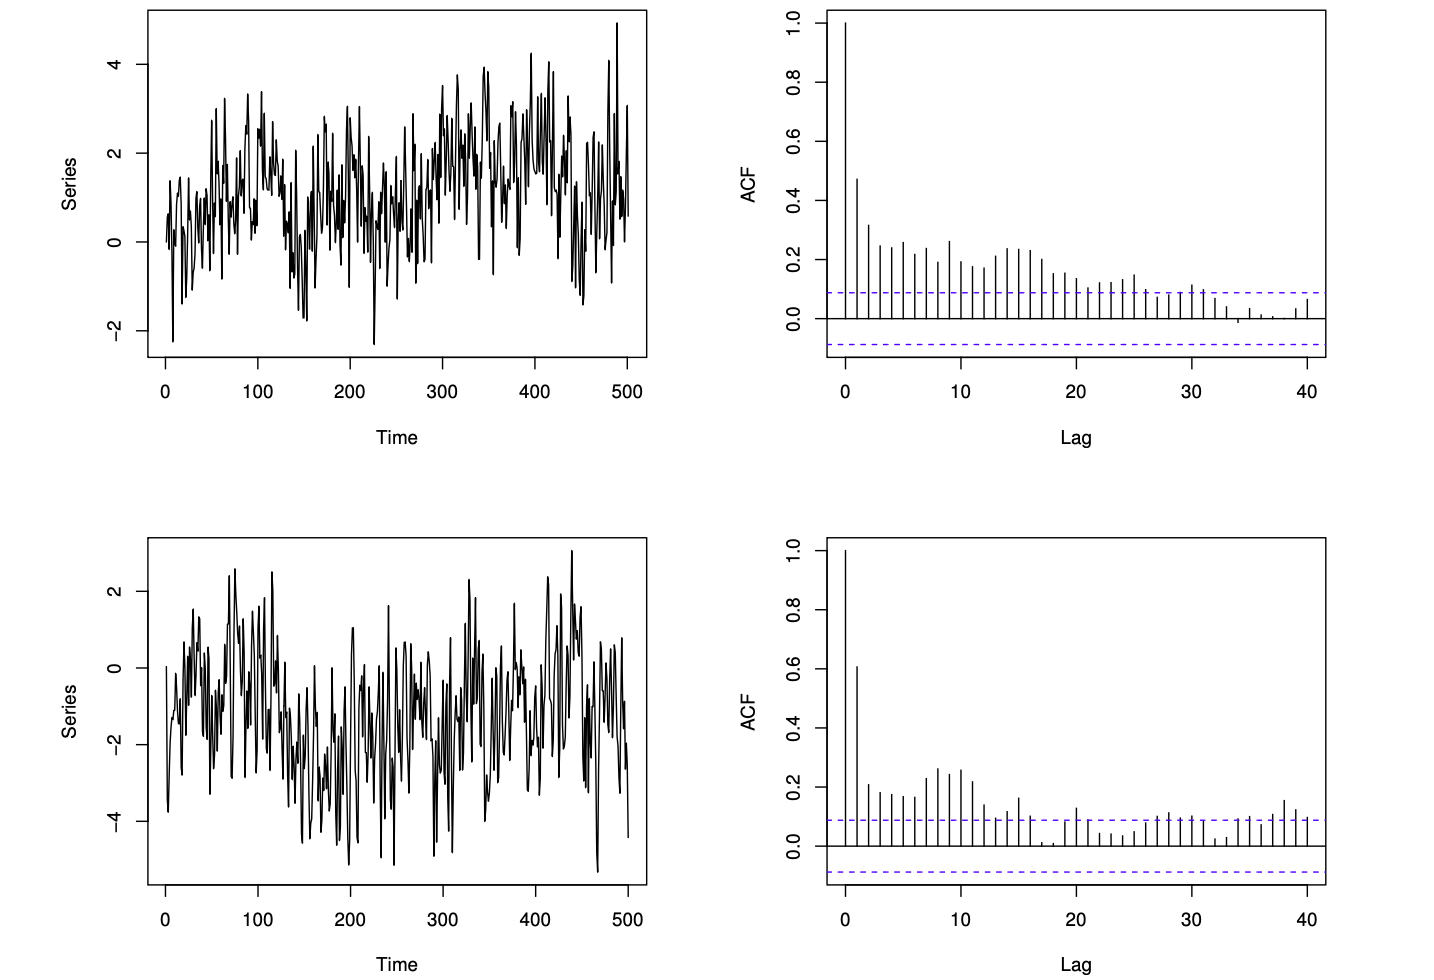
\includegraphics[width=\textwidth]{Chapter 3/fig3-9.png}
	\caption{A simulated non-stationary process and a simulated $\mathrm{ARFIMA}(1, d=0.45, 2)$ process and 
	their correlograms. Top: $(1 - 0.3B)(1 - B)X_t = (1 + 0.9B)Z_t$; Bottom: $(1 - 0.3B)(1 - B)^d X_t 
	= (1 - 0.3B + 0.5B^2) Z_t$, $Z_t \sim N(0, 1)$.}
	\label{fig:3.9}
\end{figure}

Both the series themselves and their correlograms look quite similar. Therefore, given a set of data with these 
properties which seems to be non-stationary, it may be worth considering a fractional ARIMA model with 
$0 < d < 1$, as well as an ordinary model with $d = 1$. Now the question: will the resulting forecasts likely to 
be better than those from alternative models? Currently research is still being done on this subject.



% ----------3.11----------
\subsection{The General Linear Process}
\begin{definition*}[]
A stationary process is called a \underline{general linear process} is it can be written as an MA process, i.e. 
\[ X_t = \sum_{i = 0}^{\infty} \psi_i Z_{t-i}. \]
\end{definition*}
A sufficient condition for the sum to converge, and hence for the process to be stationary, is that the 
coefficients are absolutely summable. Of course, stationary AR and ARMA processes can also be expressed as a 
general linear process using the duality between AR and MA processes.



% ----------3.12----------
\subsection{Continuous Processes}
Let's give a brief introduction in the difficulties of continuous time series.

As an example, we consider a first-order AR process in continuous time. A first order AR process in discrete 
time can be rewritten as 
\[ X_t = \alpha_{t - 1} + Z_t \implies (1 - \alpha)X_t + \alpha \nabla X_t = Z_t, \ \nabla X_t = 
(1 - B)X_t. \]
Differencing in discrete time corresponds to differentiation in continuous time, hence a natural way to define 
an AR(1) process in continuous time is via the equation 
\[ aX(t) + \frac{dX(t)}{dt} = Z(t), \]
where $a$ is a constant, and $Z(t)$ denotes continuous white noise. However, $\{ Z(t) \}$ cannot physically 
exist, hence let's rewrite the above:
\[ dX(t) = -aX(t)dt + dU(t) \]
where $\{ U(t) \}$ is a process with orthogonal increments such that the random variables $U(t_2) - U(t_1)$ and 
$U(t_4) - U(t_3)$ are uncorrelated for any two non-overlapping intervals $(t_1, t_2)$ and $(t_3, t_4)$. In the 
theory of Brownian motion, this is within the Ornstein-Uhlenbeck model and is sometimes called the Langevin 
equation. It can be shown that the process defined above has the ac.f. 
\[ \rho(\tau) = e^{-a |\tau|}, \]
which is similar to the ac.f. of an AR(1) process in discrete time in that both decay exponentially.

Rigorous studies of continuous process require considerable mathematical theory, including a knowledge of 
stochastic integration. Hence this is not covered in this book.



% ----------3.13----------
\subsection{The Wold Decomposition Theorem}
The Wold Decomposition Theorem is mostly of theoretical interest.

\begin{theorem*}[Wold's Decomposition]
Any discrete-time weakly stationary process can be expressed as the sum of a deterministic and a stochastic 
time series, i.e.
\[ X_t = \sum_{j = 0}^{\infty} b_j \varepsilon_{t - j} + \eta_t. \]
where 
\begin{itemize}
	\item $X_t$ is the time series being considered, 
	\item $\varepsilon_t$ is an uncorrelated sequence which is the innovation process of $X_t$,
	\item $b$ is the \textit{possibly infinite} vector of moving average weights, 
	\item $\eta_t$ is a deterministic time series, in the sense that it is completely determined as a linear 
	combination of its past values.	
\end{itemize}	
\end{theorem*}

While the concept of a purely indeterministic process may sometimes be helpful, the Wold decomposition itself 
can be of little assistance. For a linear purely indeterministic process like AR or ARMA, trying an 
$\mathrm{MA}(\infty)$ model is inappropriate, since there are too many parameters to estimate. For processes 
generated in a nonlinear way, the Wold decomposition is usually even of lest interest, as the best predictor 
is often nonlinear.

For example, consider 
\[ X_t = g \cos{(\omega t + \theta)}, \]
where $g$ is a constant, $\omega \in (0, \pi)$ is the frequency of the process, and $\theta \sim 
\mathrm{Unif}(0, 2 \pi)$ is a random variable, called the phase. Note that we need the term $\theta$ so that 
\[ \mathbb{E}\left[ X_t \right] = 0 \text{ for all } t. \]
If this is not done, $X_t$ will not be stationary.

As $\theta$ is fixed for a single realization, once enough value of $X_t$ have been observed to evaluate 
$\theta$, all subsequent values of $X_t$ are determined. Then we can see that $X_t$ defines a deterministic 
process. However, it is not `purely deterministic' because it is nonlinear. In fact, it is `purely stochastic' 
using a linear predictor!
